% Chapter 11 of Genesis
\bookchapter{The Tower of Babel}

\bverse Now the whole earth had one language\vmark{a} and one speech.
	\translationnote{a}{The word for `language' here (Strong's 8193 \cite{Strong's GodRules}) is distinct from the word `tongues' used in \bref{Genesis 10}. This word more literally means \textit{language} or \textit{speech}.}
	\contextnote{a}{In \bref{Genesis 10}, it makes it seem like the different lineages were separated based on their \textit{tongues}, which could mean languages. However, to be under one language here means either that \textit{tongues} specifically refers to different dialects \textit{or} that this languages is referring to something else such as the language of mathematics. We see in modern society that even though many countries have different languages, we all can write in common terms using something like mathematics. Though the `one speech' makes it seem like a more literal form of spoken language.}

\bverse And it came to pass, as they journeyed from the east, that they found a plain in the land of Shinar, and they dwelt there.
\bverse Then they said to one another, ``Come, let us make bricks and bake \textit{them} thoroughly.'' They had brick for stone, and they had asphalt for mortar.
\bverse And they said, ``Come, let us build ourselves a city, and a tower whos top \is in the heavens; let us make a name for ourselves, lest we be scattered abroad over the face of the whole earth.''
	\questionnote{}{We see here that they (the people of the time) did \textit{not} want to be scattered abroad over the face of the earth. Perhaps they knew something about sticking together that would give them an advantage? I wonder why they did not want to spread out. Perhaps they were advancing too quickly?}

\bverse But the \lord came down to see the city and the tower which the sons of men had build.
\bverse And the \lord said, ``Indeed the people \are one and they all have one language, and this is what they begin to do; now nothing that they propose to do will be withheld from them.
\bverse Come, let Us go down and there confuse their language, that they may not understand one another's speech.''
\bverse So the \lord scattered them abroad from there over the face of all the earth, and they ceased building the city.
\bverse Therefore its name is called Babel, because there the \lord confused the language of all the earth; and from there the \lord scattered them abroad over the face of all the earth.
	\questionnote{}{For some reason, the \lord decided that he had to scatter them abroad the face of the earth - which is directly opposed to what the people wanted (see \bref{Genesis 11:4}). Why did he find the need or desire to do this?}

\bmarkerdown{\name{Shem}'s Descendants}

\bverse This \is the genealogy of \name{Shem}: \name{Shem} was one hundred years old, and begot \name{Arphaxad} two years after the flood.
\bverse After he begot \name{Arphaxad}, \name{Shem} lived five hundred years, and begot sons and daughters.
\bverse \name{Arphaxad} lived thirty-five years, and begot \name{Salah}.
\bverse After he begot \name{Salah}, \name{Arphaxad} lived four hundred and three years, and begot sons and daughters.
\bverse \name{Salah} lived thirty years, and begot \name{Eber}.
\bverse After he begot \name{Eber}, \name{Salah} lived four hundred and three years, and begot sons and daughters.
\bverse \name{Eber} lived thirty-four years, and begot \name{Peleg}.
\bverse After he begot \name{Peleg}, \name{Eber} lived four hundred and thirty years, and begot sons and daughters.
\bverse \name{Peleg} lived thirty years, and begot \name{Reu}. 
\bverse After he begot \name{Reu}, \name{Peleg} lived two hundred and nine years, and begot sons and daughters.
\bverse \name{Reu} lived thirty-two years, and begot \name{Serug}.
\bverse After he begot \name{Serug}, \name{Reu} lived two hundred and seven years, and begot sons and daughters.
\bverse \name{Serug} lived thirty years, and begot \name{Nahor}.
\bverse After he begot \name{Nahor}, \name{Serug} lived two hundred years, and begot sons and daughters.
\bverse \name{Nahor} lived twenty-nine years, and begot \name{Terah}.
\bverse After he begot \name{Terah}, \name{Nahor} lived one hundred and nineteen years, and begot sons and daughters.
\bverse Now \name{Terah} lived seventy years, and begot \name{Abram}, \name{Nahor}, and \name{Haran}.



\begin{figure}[h] % h=here
	\centering
	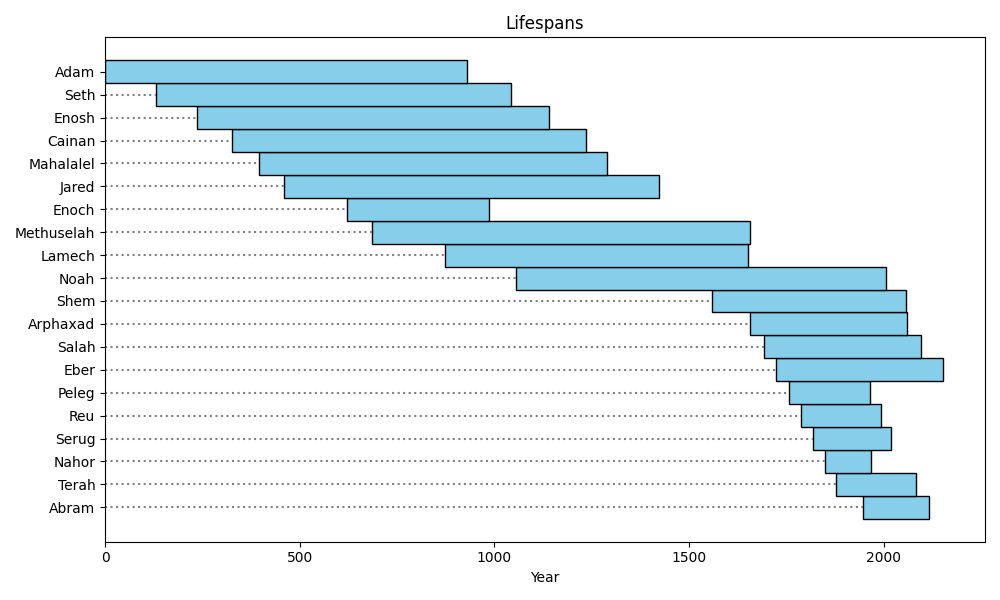
\includegraphics[width=0.95\linewidth]{images/lifespans/pre_abram_lifespans.png}
	\caption{This chart shows the lifespans of various individuals whose total lifespans are mentioned. The chart covers individuals up to and including \name{Abram}.}
	\label{fig:pre_adam_lifespans}
\end{figure}



\bmarkerdown{\name{Terah}'s Descendants}

\bverse This is the genealogy of \name{Terah}: \name{Terah} begot \name{Abram}, \name{Nahor}, and \name{Haran}. \name{Haran} begot \name{Lot}.
\bverse And \name{Haran} died before his father \name{Terah} in his native land, in Ur of the Chaldeans.
\bverse Then \name{Abram} and \name{Nahor} took wives: the name of \name{Abram}'s wife \was \name{Sarai}, and the name of \name{Nahor}'s wife, \name{Milcah}, the daughter of \name{Haran} the father of \name{Milcah} and the father of \name{Iscah}.
\bverse But \name{Sarai} was barren; she had no child.
\bverse And \name{Terah} took his son \name{Abram} and his grandson \name{Lot}, the son of \name{Haran}, and his daughter-in-law \name{Sarai}, his son \name{Abram}'s wife, and they went out with them from Ur of the Chaldeans to go to the land of Canaan; and they came to Haran and dwelt there.
\bverse So the days of \name{Terah} were two hundred and five years, and \name{Terah} died in Haran.



\begin{figure}[htbp] % h=here, t=top, b=bottom, p=page
	\centering
	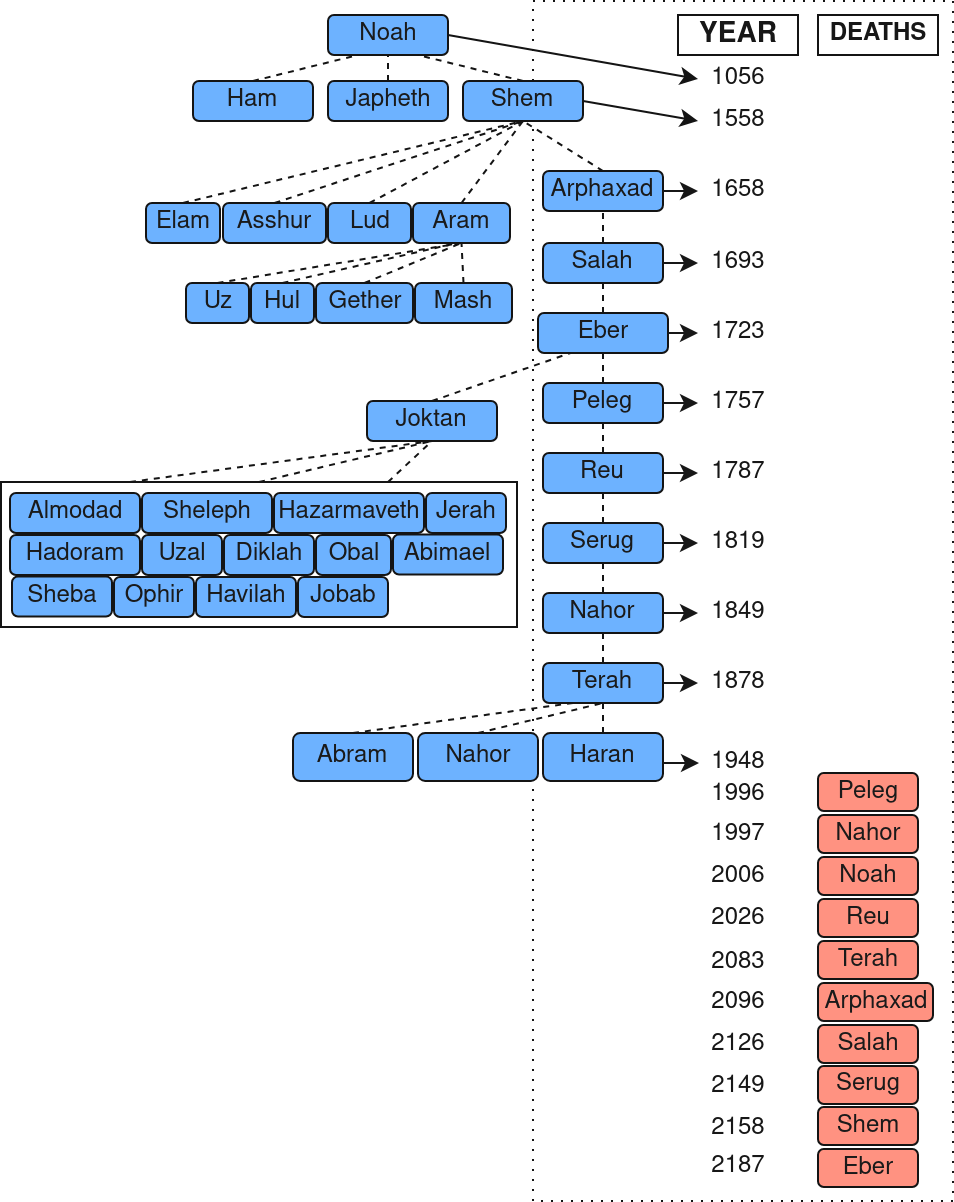
\includegraphics[width=0.9\linewidth]{images/genealogies/shems_genealogy.png}
	\caption{This is a diagram showing the genealogy of the family of \name{Shem} as outlined in \bref{Genesis 10} and \bref{Genesis 11}. It ends with \name{Terah}'s three children (\name{Abram}, \name{Nahor}, and \name{Haran}) from \bref{Genesis 11:26}. Males are depicted in blue. The genealogy shows timeline markers showing the year of birth and death for many of the descendants (where outlined in \bref{Genesis 11}), which are primarily in the dotted box. The box with a bold border represents all the sons of \name{Joktan}. This diagram was created by me using the draw.io tool \cite{draw.io}.}
	\label{fig:shems_genealogy}
\end{figure}
